% Options for packages loaded elsewhere
\PassOptionsToPackage{unicode}{hyperref}
\PassOptionsToPackage{hyphens}{url}
\PassOptionsToPackage{dvipsnames,svgnames,x11names}{xcolor}
%
\documentclass[
  letterpaper,
  DIV=11,
  numbers=noendperiod]{scrartcl}

\usepackage{amsmath,amssymb}
\usepackage{iftex}
\ifPDFTeX
  \usepackage[T1]{fontenc}
  \usepackage[utf8]{inputenc}
  \usepackage{textcomp} % provide euro and other symbols
\else % if luatex or xetex
  \usepackage{unicode-math}
  \defaultfontfeatures{Scale=MatchLowercase}
  \defaultfontfeatures[\rmfamily]{Ligatures=TeX,Scale=1}
\fi
\usepackage{lmodern}
\ifPDFTeX\else  
    % xetex/luatex font selection
\fi
% Use upquote if available, for straight quotes in verbatim environments
\IfFileExists{upquote.sty}{\usepackage{upquote}}{}
\IfFileExists{microtype.sty}{% use microtype if available
  \usepackage[]{microtype}
  \UseMicrotypeSet[protrusion]{basicmath} % disable protrusion for tt fonts
}{}
\makeatletter
\@ifundefined{KOMAClassName}{% if non-KOMA class
  \IfFileExists{parskip.sty}{%
    \usepackage{parskip}
  }{% else
    \setlength{\parindent}{0pt}
    \setlength{\parskip}{6pt plus 2pt minus 1pt}}
}{% if KOMA class
  \KOMAoptions{parskip=half}}
\makeatother
\usepackage{xcolor}
\setlength{\emergencystretch}{3em} % prevent overfull lines
\setcounter{secnumdepth}{-\maxdimen} % remove section numbering
% Make \paragraph and \subparagraph free-standing
\ifx\paragraph\undefined\else
  \let\oldparagraph\paragraph
  \renewcommand{\paragraph}[1]{\oldparagraph{#1}\mbox{}}
\fi
\ifx\subparagraph\undefined\else
  \let\oldsubparagraph\subparagraph
  \renewcommand{\subparagraph}[1]{\oldsubparagraph{#1}\mbox{}}
\fi

\usepackage{color}
\usepackage{fancyvrb}
\newcommand{\VerbBar}{|}
\newcommand{\VERB}{\Verb[commandchars=\\\{\}]}
\DefineVerbatimEnvironment{Highlighting}{Verbatim}{commandchars=\\\{\}}
% Add ',fontsize=\small' for more characters per line
\usepackage{framed}
\definecolor{shadecolor}{RGB}{241,243,245}
\newenvironment{Shaded}{\begin{snugshade}}{\end{snugshade}}
\newcommand{\AlertTok}[1]{\textcolor[rgb]{0.68,0.00,0.00}{#1}}
\newcommand{\AnnotationTok}[1]{\textcolor[rgb]{0.37,0.37,0.37}{#1}}
\newcommand{\AttributeTok}[1]{\textcolor[rgb]{0.40,0.45,0.13}{#1}}
\newcommand{\BaseNTok}[1]{\textcolor[rgb]{0.68,0.00,0.00}{#1}}
\newcommand{\BuiltInTok}[1]{\textcolor[rgb]{0.00,0.23,0.31}{#1}}
\newcommand{\CharTok}[1]{\textcolor[rgb]{0.13,0.47,0.30}{#1}}
\newcommand{\CommentTok}[1]{\textcolor[rgb]{0.37,0.37,0.37}{#1}}
\newcommand{\CommentVarTok}[1]{\textcolor[rgb]{0.37,0.37,0.37}{\textit{#1}}}
\newcommand{\ConstantTok}[1]{\textcolor[rgb]{0.56,0.35,0.01}{#1}}
\newcommand{\ControlFlowTok}[1]{\textcolor[rgb]{0.00,0.23,0.31}{#1}}
\newcommand{\DataTypeTok}[1]{\textcolor[rgb]{0.68,0.00,0.00}{#1}}
\newcommand{\DecValTok}[1]{\textcolor[rgb]{0.68,0.00,0.00}{#1}}
\newcommand{\DocumentationTok}[1]{\textcolor[rgb]{0.37,0.37,0.37}{\textit{#1}}}
\newcommand{\ErrorTok}[1]{\textcolor[rgb]{0.68,0.00,0.00}{#1}}
\newcommand{\ExtensionTok}[1]{\textcolor[rgb]{0.00,0.23,0.31}{#1}}
\newcommand{\FloatTok}[1]{\textcolor[rgb]{0.68,0.00,0.00}{#1}}
\newcommand{\FunctionTok}[1]{\textcolor[rgb]{0.28,0.35,0.67}{#1}}
\newcommand{\ImportTok}[1]{\textcolor[rgb]{0.00,0.46,0.62}{#1}}
\newcommand{\InformationTok}[1]{\textcolor[rgb]{0.37,0.37,0.37}{#1}}
\newcommand{\KeywordTok}[1]{\textcolor[rgb]{0.00,0.23,0.31}{#1}}
\newcommand{\NormalTok}[1]{\textcolor[rgb]{0.00,0.23,0.31}{#1}}
\newcommand{\OperatorTok}[1]{\textcolor[rgb]{0.37,0.37,0.37}{#1}}
\newcommand{\OtherTok}[1]{\textcolor[rgb]{0.00,0.23,0.31}{#1}}
\newcommand{\PreprocessorTok}[1]{\textcolor[rgb]{0.68,0.00,0.00}{#1}}
\newcommand{\RegionMarkerTok}[1]{\textcolor[rgb]{0.00,0.23,0.31}{#1}}
\newcommand{\SpecialCharTok}[1]{\textcolor[rgb]{0.37,0.37,0.37}{#1}}
\newcommand{\SpecialStringTok}[1]{\textcolor[rgb]{0.13,0.47,0.30}{#1}}
\newcommand{\StringTok}[1]{\textcolor[rgb]{0.13,0.47,0.30}{#1}}
\newcommand{\VariableTok}[1]{\textcolor[rgb]{0.07,0.07,0.07}{#1}}
\newcommand{\VerbatimStringTok}[1]{\textcolor[rgb]{0.13,0.47,0.30}{#1}}
\newcommand{\WarningTok}[1]{\textcolor[rgb]{0.37,0.37,0.37}{\textit{#1}}}

\providecommand{\tightlist}{%
  \setlength{\itemsep}{0pt}\setlength{\parskip}{0pt}}\usepackage{longtable,booktabs,array}
\usepackage{calc} % for calculating minipage widths
% Correct order of tables after \paragraph or \subparagraph
\usepackage{etoolbox}
\makeatletter
\patchcmd\longtable{\par}{\if@noskipsec\mbox{}\fi\par}{}{}
\makeatother
% Allow footnotes in longtable head/foot
\IfFileExists{footnotehyper.sty}{\usepackage{footnotehyper}}{\usepackage{footnote}}
\makesavenoteenv{longtable}
\usepackage{graphicx}
\makeatletter
\def\maxwidth{\ifdim\Gin@nat@width>\linewidth\linewidth\else\Gin@nat@width\fi}
\def\maxheight{\ifdim\Gin@nat@height>\textheight\textheight\else\Gin@nat@height\fi}
\makeatother
% Scale images if necessary, so that they will not overflow the page
% margins by default, and it is still possible to overwrite the defaults
% using explicit options in \includegraphics[width, height, ...]{}
\setkeys{Gin}{width=\maxwidth,height=\maxheight,keepaspectratio}
% Set default figure placement to htbp
\makeatletter
\def\fps@figure{htbp}
\makeatother

\KOMAoption{captions}{tableheading}
\makeatletter
\@ifpackageloaded{tcolorbox}{}{\usepackage[skins,breakable]{tcolorbox}}
\@ifpackageloaded{fontawesome5}{}{\usepackage{fontawesome5}}
\definecolor{quarto-callout-color}{HTML}{909090}
\definecolor{quarto-callout-note-color}{HTML}{0758E5}
\definecolor{quarto-callout-important-color}{HTML}{CC1914}
\definecolor{quarto-callout-warning-color}{HTML}{EB9113}
\definecolor{quarto-callout-tip-color}{HTML}{00A047}
\definecolor{quarto-callout-caution-color}{HTML}{FC5300}
\definecolor{quarto-callout-color-frame}{HTML}{acacac}
\definecolor{quarto-callout-note-color-frame}{HTML}{4582ec}
\definecolor{quarto-callout-important-color-frame}{HTML}{d9534f}
\definecolor{quarto-callout-warning-color-frame}{HTML}{f0ad4e}
\definecolor{quarto-callout-tip-color-frame}{HTML}{02b875}
\definecolor{quarto-callout-caution-color-frame}{HTML}{fd7e14}
\makeatother
\makeatletter
\makeatother
\makeatletter
\makeatother
\makeatletter
\@ifpackageloaded{caption}{}{\usepackage{caption}}
\AtBeginDocument{%
\ifdefined\contentsname
  \renewcommand*\contentsname{Table of contents}
\else
  \newcommand\contentsname{Table of contents}
\fi
\ifdefined\listfigurename
  \renewcommand*\listfigurename{List of Figures}
\else
  \newcommand\listfigurename{List of Figures}
\fi
\ifdefined\listtablename
  \renewcommand*\listtablename{List of Tables}
\else
  \newcommand\listtablename{List of Tables}
\fi
\ifdefined\figurename
  \renewcommand*\figurename{Figure}
\else
  \newcommand\figurename{Figure}
\fi
\ifdefined\tablename
  \renewcommand*\tablename{Table}
\else
  \newcommand\tablename{Table}
\fi
}
\@ifpackageloaded{float}{}{\usepackage{float}}
\floatstyle{ruled}
\@ifundefined{c@chapter}{\newfloat{codelisting}{h}{lop}}{\newfloat{codelisting}{h}{lop}[chapter]}
\floatname{codelisting}{Listing}
\newcommand*\listoflistings{\listof{codelisting}{List of Listings}}
\makeatother
\makeatletter
\@ifpackageloaded{caption}{}{\usepackage{caption}}
\@ifpackageloaded{subcaption}{}{\usepackage{subcaption}}
\makeatother
\makeatletter
\@ifpackageloaded{tcolorbox}{}{\usepackage[skins,breakable]{tcolorbox}}
\makeatother
\makeatletter
\@ifundefined{shadecolor}{\definecolor{shadecolor}{rgb}{.97, .97, .97}}
\makeatother
\makeatletter
\makeatother
\makeatletter
\makeatother
\ifLuaTeX
  \usepackage{selnolig}  % disable illegal ligatures
\fi
\IfFileExists{bookmark.sty}{\usepackage{bookmark}}{\usepackage{hyperref}}
\IfFileExists{xurl.sty}{\usepackage{xurl}}{} % add URL line breaks if available
\urlstyle{same} % disable monospaced font for URLs
\hypersetup{
  pdftitle={Problem Set 01: Intro to R and RStudio},
  pdfauthor={Your Name Goes Here},
  colorlinks=true,
  linkcolor={blue},
  filecolor={Maroon},
  citecolor={Blue},
  urlcolor={Blue},
  pdfcreator={LaTeX via pandoc}}

\title{Problem Set 01: Intro to R and RStudio}
\author{Your Name Goes Here}
\date{Last modified on July 31, 2023 15:09:35 Eastern Daylight Time}

\begin{document}
\maketitle
\ifdefined\Shaded\renewenvironment{Shaded}{\begin{tcolorbox}[interior hidden, sharp corners, frame hidden, boxrule=0pt, breakable, borderline west={3pt}{0pt}{shadecolor}, enhanced]}{\end{tcolorbox}}\fi

\begin{center}\rule{0.5\linewidth}{0.5pt}\end{center}

\begin{figure}

{\centering 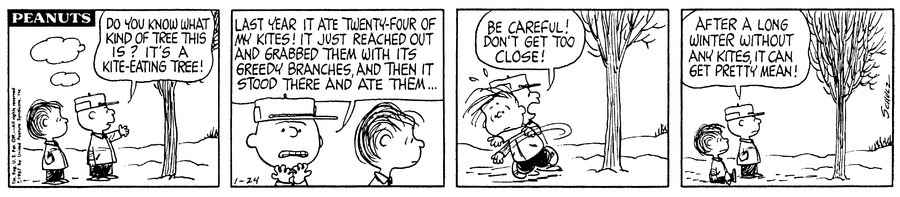
\includegraphics[width=7.14in,height=\textheight]{./figures/cbrown.jpg}

}

\end{figure}

The goal this week is to introduce \texttt{R} and RStudio which will be
used throughout the course both to review the statistical concepts
discussed in the course and to analyze real data and come to informed
conclusions. To clarify which is which: \texttt{R} is the name of the
programming language itself, and RStudio is an integrated development
editor (IDE).

Today, we begin with the fundamental building blocks of \texttt{R} and
RStudio: the interface, creating and saving files, and basic commands.

\begin{center}\rule{0.5\linewidth}{0.5pt}\end{center}

\hypertarget{opening-rstudio-server}{%
\section{Opening RStudio Server}\label{opening-rstudio-server}}

Open Appalachian's RStudio Server and sign in:
\href{https://mathr.appstate.edu}{RStudio Server}

Your credentials are the same ones you use to log into your ASU email
account.

Please \textbf{DO NOT} choose Stay signed in.

\begin{Shaded}
\begin{Highlighting}[]

\end{Highlighting}
\end{Shaded}

\begin{center}\rule{0.5\linewidth}{0.5pt}\end{center}

\hypertarget{the-rstudio-interface}{%
\section{The RStudio Interface}\label{the-rstudio-interface}}

In the RStudio Server, you should see a window that looks like the image
in Figure~\ref{fig-rstudio}.

\begin{figure}

{\centering 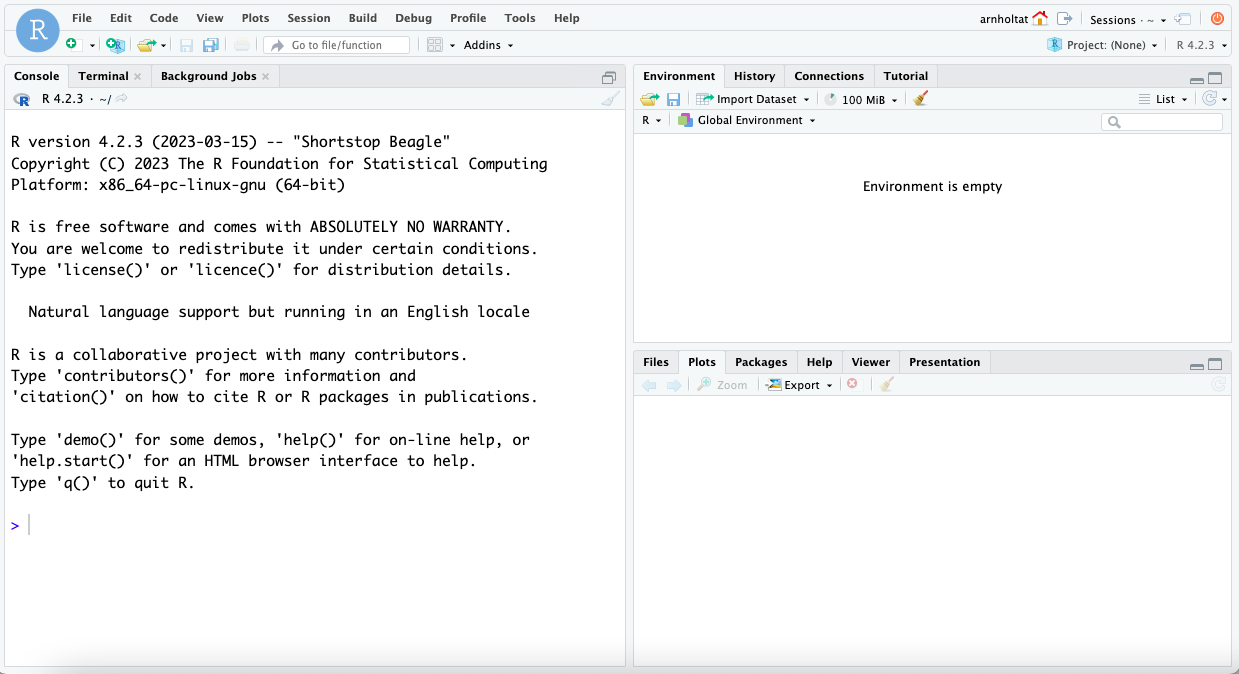
\includegraphics[width=9.83in,height=\textheight]{./figures/RStudio-Opening.png}

}

\caption{\label{fig-rstudio}The RStudio interface}

\end{figure}

The panel on the left is where the action happens. It's called the
\textbf{\emph{console}}. Every time RStudio is launched, it will have
the same text at the top of the console describing the version of
\texttt{R} that is running.

The panel in the upper right contains the \textbf{\emph{workspace}}.
This shows the variables and objects defined during an \texttt{R}
session and a history of the commands that are entered.

Any plots that are generated will show up in the panel in the lower
right corner. This is also where you can browse your files, access help
files, and upload and download files.

\begin{center}\rule{0.5\linewidth}{0.5pt}\end{center}

\hypertarget{using-quarto-files}{%
\section{Using Quarto Files}\label{using-quarto-files}}

At its core, Quarto works the same way as R Markdown:

\begin{figure}[H]

{\centering 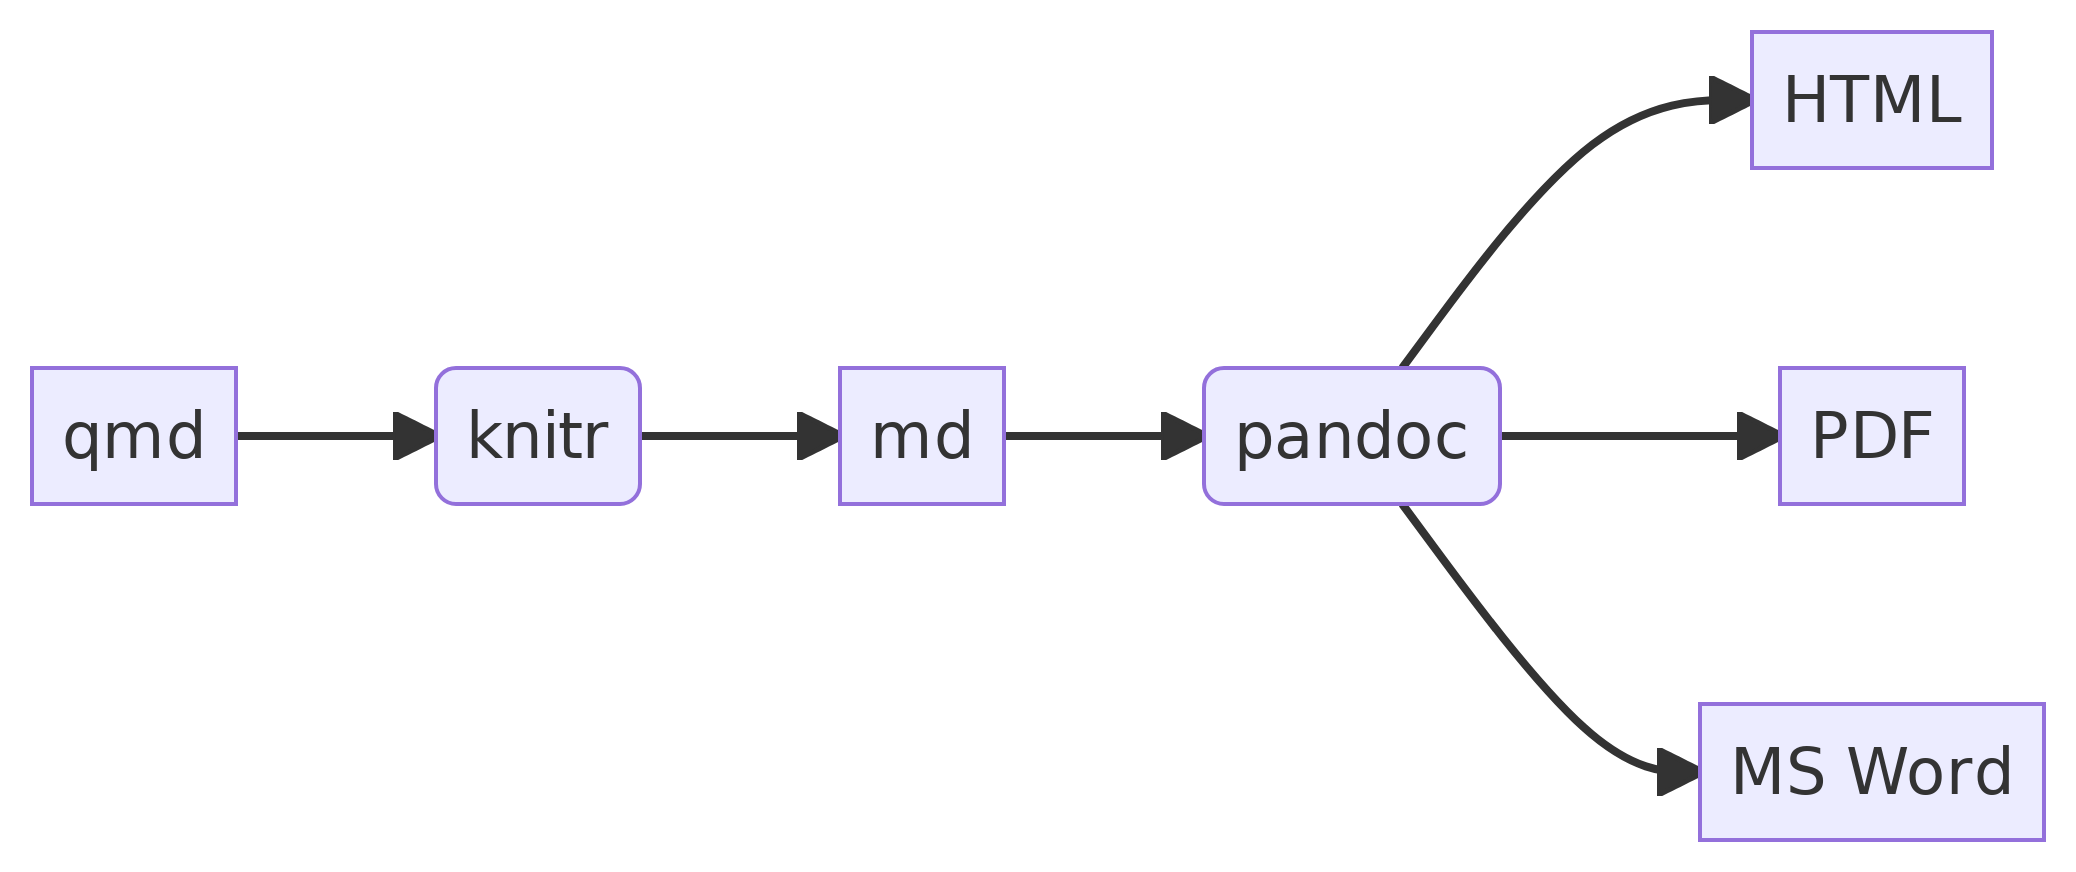
\includegraphics[width=5.41in,height=2.27in]{PS01_source_files/figure-latex/mermaid-figure-1.png}

}

\end{figure}

Quarto combines the functionality of R Markdown, bookdown, distill,
xaringian, etc. into a single consistent system. Quarto is at its core
multi-language and multi-engine (supporting Knitr, Jupyter, and
Observable today and potentially other engines tomorrow).

\hypertarget{opening-a-new-file}{%
\subsection{Opening a New File}\label{opening-a-new-file}}

Quarto documents can be used in \texttt{R} or python. For this course,
we will use \texttt{R} and the RStudio IDE to work with Quarto
documents. Quarto documents are useful for both running code and
annotating the code with comments. The documents can be saved, so you
can refer back to your code later. Quarto documents can also be used to
generate other document types (HTML, PDF, MS Word, Open Office, or ePub)
for presenting the results of your analyses in formats that may be
required in other contexts.

To open a new Quarto document, click on the little green plus beside the
circled R in the upper left hand area of the RStudio IDE as seen in
Figure~\ref{fig-rstudio} and select \texttt{Quarto\ Document...}. Enter
a title and author in the corresponding boxes; then, click create. See
Figure~\ref{fig-open} for an example where the document title is
\textbf{Something Cool} and the author is \textbf{Joe Quarto}.

\begin{figure}

{\centering 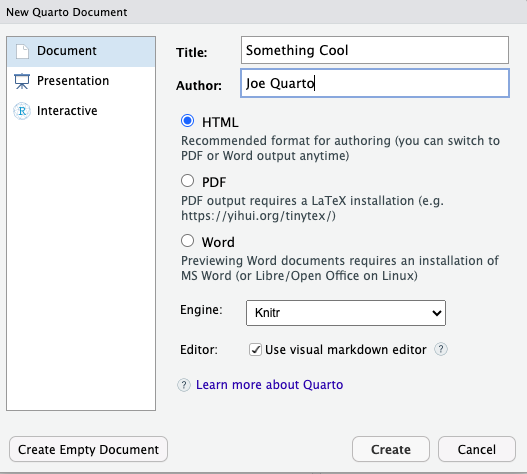
\includegraphics[width=4.15in,height=\textheight]{figures/open-QUARTO.png}

}

\caption{\label{fig-open}Starting a new Quarto document}

\end{figure}

When you open a new Quarto document, there is some example code
(template) in it that you might delete.

\hypertarget{saving-a-file}{%
\subsection{Saving a File}\label{saving-a-file}}

Lab work will be saved as Quarto files that will be committed and pushed
to the class repository. Therefore, it is important to learn how to save
these files. To save the Quarto template:

\begin{itemize}
\tightlist
\item
  Click File \textgreater{} Save As\ldots{}
\item
  Name the file: \texttt{PS01\_YourLastName\_YourFirstName} (mine would
  be \texttt{PS01\_Arnholt\_Alan.qmd}).
\end{itemize}

\begin{tcolorbox}[enhanced jigsaw, titlerule=0mm, toprule=.15mm, arc=.35mm, colbacktitle=quarto-callout-warning-color!10!white, coltitle=black, colframe=quarto-callout-warning-color-frame, left=2mm, breakable, bottomtitle=1mm, toptitle=1mm, bottomrule=.15mm, title=\textcolor{quarto-callout-warning-color}{\faExclamationTriangle}\hspace{0.5em}{Warning}, colback=white, rightrule=.15mm, opacityback=0, opacitybacktitle=0.6, leftrule=.75mm]

The \texttt{PS01\_YourLastName\_YourFirstName.qmd} file is just for your
own practice. The file you will save, commit, and push to the class
repository is the file you are reading (\texttt{PS01\_source.qmd}). You
will make changes to this file starting in
Section~\ref{sec-practice-on-your-own} (Practice on Your Own).

\end{tcolorbox}

\begin{itemize}
\tightlist
\item
  Click save. The \texttt{PS01\_YourLastName\_YourFirstName.qmd} is now
  saved in the \texttt{MD-PS01-SC} directory \textbf{on the server}.
\end{itemize}

\hypertarget{make-changes-to-a-file}{%
\subsection{Make Changes to a File}\label{make-changes-to-a-file}}

Let's make some changes to the Quarto document you just created using
Figure~\ref{fig-changes} as a guide.

\begin{itemize}
\item
  First, change the title of the document to \textbf{Using the RStudio
  IDE with Quarto}. Be sure to surround the title with quotation marks.
\item
  Second, add your name to the author field, making sure to include your
  name inside quotation marks.
\item
  Third, click on \texttt{Source} in the upper left of the
  \texttt{*.qmd} source's panel so that line numbers appear on the far
  left.
\item
  Fourth, delete lines 12 through 27.
\item
  Finally, insert what is called a ``code chunk.'' To do this, click on
  the green +C (insert a new code chunk) button near the top right of
  the \texttt{*.qmd} source's panel. \texttt{R} code is entered on the
  blank line inside the \texttt{R} code chunk.
\end{itemize}

Your final result should look similar to Figure~\ref{fig-changes}.

\begin{figure}

{\centering 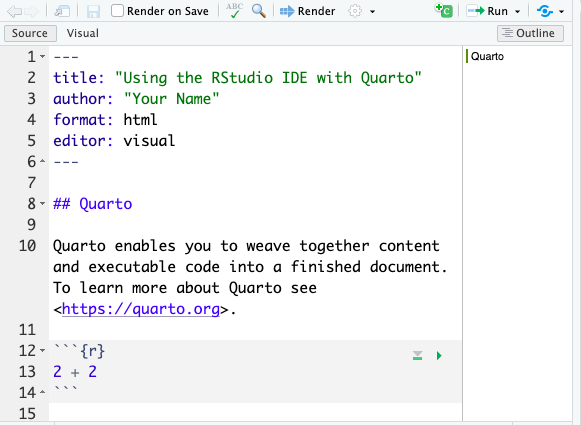
\includegraphics[width=4.57in,height=\textheight]{figures/QUATRO-changes.png}

}

\caption{\label{fig-changes}Quarto source file}

\end{figure}

\hypertarget{rendering-a-file}{%
\subsection{Rendering a File}\label{rendering-a-file}}

Click the \(\Rightarrow\) Render button at the top left side of the
screen to ``render'' the file, or in other words, produce a formatted
document. An \texttt{*.html} file will be generated. The \texttt{*.html}
file is automatically saved in the same folder as your Quarto file.

Note that there are now a Quarto file
(\texttt{PS01\_YourLastName\_YourFirstName.qmd}) and an html file
(\texttt{PS01\_lastname\_firstname.html}) in the \texttt{MD-PS01-SC}
folder in addition to the files you downloaded.

Inspect the \texttt{*.html} file to see how what you typed was
formatted. There are lots of tricks for controlling the formatting of
the rendered html file. For instance:

\begin{itemize}
\tightlist
\item
  putting \texttt{\#\#} and a space in front of text makes it into a
  large header. For example, see how \texttt{\#\#\ This\ is\ a\ header}
  in your Quarto \texttt{*.qmd} file translates in the resulting
  \texttt{*.html} output.
\item
  putting \texttt{\#\#\#} and a space in front of text makes it a
  smaller header.
\end{itemize}

\begin{center}\rule{0.5\linewidth}{0.5pt}\end{center}

\hypertarget{entering-and-running-commands}{%
\section{Entering and Running
Commands}\label{entering-and-running-commands}}

The code chunks are where you put \texttt{R} code in Quarto file. So
far, your ``rendered'' file (your formatted document file) doesn't show
anything because we did not put any content in the code chunks yet.

Using your first code chunk, type the following command to create a new
variable called \texttt{x} with the value of 6.

\begin{Shaded}
\begin{Highlighting}[]
\NormalTok{x }\OtherTok{\textless{}{-}} \DecValTok{6}
\end{Highlighting}
\end{Shaded}

The arrow \texttt{\textless{}-} is called an \textbf{\emph{assignment
operator}} and tells \texttt{R} to save an object called \texttt{x} that
has the value of 6. This is similar to saving a value in a graphing
calculator.

\begin{tcolorbox}[enhanced jigsaw, titlerule=0mm, toprule=.15mm, arc=.35mm, colbacktitle=quarto-callout-tip-color!10!white, coltitle=black, colframe=quarto-callout-tip-color-frame, left=2mm, breakable, bottomtitle=1mm, toptitle=1mm, bottomrule=.15mm, title=\textcolor{quarto-callout-tip-color}{\faLightbulb}\hspace{0.5em}{Tip}, colback=white, rightrule=.15mm, opacityback=0, opacitybacktitle=0.6, leftrule=.75mm]

Note that whatever you want to save must always be to the left of the
assignment operator (\texttt{\textless{}-}).

\end{tcolorbox}

To \textbf{\emph{run}} this command in your console, you have a few
options:

\begin{itemize}
\tightlist
\item
  Click on the green triangle in the first line of the code chunk that
  points to the right.
\item
  Highlight the code and hit \texttt{Control-Enter} on a PC or
  \texttt{Command-Return} on a Mac.
\end{itemize}

Think of ``running'' code in your console as telling \texttt{R} ``do
this.''

Note that you now have a new object in your workspace, called
\texttt{x}.

\begin{figure}

{\centering 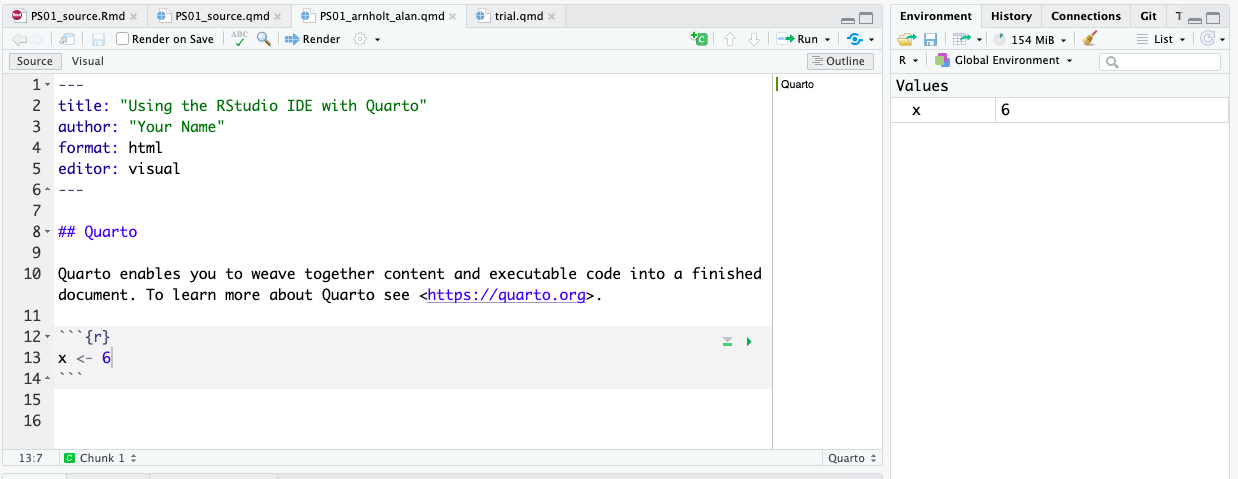
\includegraphics[width=9.75in,height=\textheight]{figures/quarto-workspace.png}

}

\end{figure}

\begin{center}\rule{0.5\linewidth}{0.5pt}\end{center}

\hypertarget{data-types-a-brief-intro}{%
\section{\texorpdfstring{Data Types\(-\)a Brief
Intro}{Data Types-a Brief Intro}}\label{data-types-a-brief-intro}}

So far, you have made a numeric variable \texttt{x}. There many other
types of data objects you can make in \texttt{R}. In this section, we
create different types of objects.

To make a \textbf{character} object called \texttt{favorite\_movie}
copy, paste, and run the following code in a new code chunk. Think of
characters as text as opposed to numerical values. Note that \texttt{R}
knows this is a \textbf{character} because there are quotation marks
around \texttt{Star\_Wars}.

\begin{Shaded}
\begin{Highlighting}[]
\NormalTok{favorite\_movie }\OtherTok{\textless{}{-}} \StringTok{"Star\_Wars"}
\end{Highlighting}
\end{Shaded}

Next, copy, paste, and run the following command in a new code chunk.

\begin{Shaded}
\begin{Highlighting}[]
\NormalTok{v }\OtherTok{\textless{}{-}} \FunctionTok{c}\NormalTok{(}\DecValTok{2}\NormalTok{, }\DecValTok{4}\NormalTok{, }\DecValTok{6}\NormalTok{)}
\end{Highlighting}
\end{Shaded}

This makes what is called a \textbf{vector}, which we have named
\texttt{v}. It is a data object that has multiple elements of the same
type. This vector contains three numbers: 2, 4, and 6. The \texttt{c()}
function says tells \texttt{R} to \texttt{concatenate} the values 2, 4,
6, into a single \textbf{vector}. Note in the Environment pane that your
vector \texttt{v} contains numbers (listed as \texttt{num}).

You can do math on a vector that contains numbers. For instance, copy,
paste, and run the following command in a new code chunk. This tells R
to multiply each element of the vector \texttt{v} by 3.

\begin{Shaded}
\begin{Highlighting}[]
\NormalTok{v }\SpecialCharTok{*} \DecValTok{3}
\end{Highlighting}
\end{Shaded}

\begin{center}\rule{0.5\linewidth}{0.5pt}\end{center}

\hypertarget{sec-practice-on-your-own}{%
\section{Practice on Your Own}\label{sec-practice-on-your-own}}

\begin{tcolorbox}[enhanced jigsaw, titlerule=0mm, toprule=.15mm, arc=.35mm, colbacktitle=quarto-callout-warning-color!10!white, coltitle=black, colframe=quarto-callout-warning-color-frame, left=2mm, breakable, bottomtitle=1mm, toptitle=1mm, bottomrule=.15mm, title=\textcolor{quarto-callout-warning-color}{\faExclamationTriangle}\hspace{0.5em}{Directions}, colback=white, rightrule=.15mm, opacityback=0, opacitybacktitle=0.6, leftrule=.75mm]

Type complete sentences to answer all questions in the Quarto document.
Round all numeric answers you report to four decimal places. Use inline
\texttt{R} code to report all numeric answers (i.e.~do not hard code
your numeric answers).

Remember to save your work as you go along. Click the floppy disk (save
current document) button in the upper left hand corner of the Quarto
source panel.

\end{tcolorbox}

\begin{center}\rule{0.5\linewidth}{0.5pt}\end{center}

\begin{tcolorbox}[enhanced jigsaw, titlerule=0mm, toprule=.15mm, arc=.35mm, colbacktitle=quarto-callout-note-color!10!white, coltitle=black, colframe=quarto-callout-note-color-frame, left=2mm, breakable, bottomtitle=1mm, toptitle=1mm, bottomrule=.15mm, title={Problem 1}, colback=white, rightrule=.15mm, opacityback=0, opacitybacktitle=0.6, leftrule=.75mm]

Answer the following with code in a code chunk (no text necessary).
Remember that the code is just \textbf{instructions} for \texttt{R}. You
need to run the code chunk to make \texttt{R} execute those
instructions.

\begin{itemize}
\tightlist
\item
  Create an empty code chunk and click on the Run all previous code
  chunks.
\item
  Create a variable called \texttt{y} with the value of 7.
\item
  Multiply \texttt{x} by \texttt{y}, and store the answer in a variable
  named \texttt{z} like so: \texttt{z\ \textless{}-\ x\ *\ y}.
\item
  Run the current code chunk, and you should now see
  \texttt{favorite\_movie}, \texttt{x}, \texttt{v}, \texttt{y}, and
  \texttt{z} all in your Environment pane.
\end{itemize}

\end{tcolorbox}

\begin{tcolorbox}[enhanced jigsaw, titlerule=0mm, toprule=.15mm, arc=.35mm, colbacktitle=quarto-callout-important-color!10!white, coltitle=black, colframe=quarto-callout-important-color-frame, left=2mm, breakable, bottomtitle=1mm, toptitle=1mm, bottomrule=.15mm, title={Problem 1 Answers}, colback=white, rightrule=.15mm, opacityback=0, opacitybacktitle=0.6, leftrule=.75mm]

\begin{Shaded}
\begin{Highlighting}[]
\CommentTok{\# Type your code and comments inside the code chunk}
\end{Highlighting}
\end{Shaded}

\end{tcolorbox}

\begin{tcolorbox}[enhanced jigsaw, titlerule=0mm, toprule=.15mm, arc=.35mm, colbacktitle=quarto-callout-note-color!10!white, coltitle=black, colframe=quarto-callout-note-color-frame, left=2mm, breakable, bottomtitle=1mm, toptitle=1mm, bottomrule=.15mm, title={Problem 2}, colback=white, rightrule=.15mm, opacityback=0, opacitybacktitle=0.6, leftrule=.75mm]

\begin{itemize}
\tightlist
\item
  Run the following mathematical operation in a code chunk:
  \texttt{6\ +\ 3}
\item
  Where does the answer appear? (please answer with \textbf{text})
\end{itemize}

\end{tcolorbox}

\begin{tcolorbox}[enhanced jigsaw, titlerule=0mm, toprule=.15mm, arc=.35mm, colbacktitle=quarto-callout-important-color!10!white, coltitle=black, colframe=quarto-callout-important-color-frame, left=2mm, breakable, bottomtitle=1mm, toptitle=1mm, bottomrule=.15mm, title={Problem 2 Answers}, colback=white, rightrule=.15mm, opacityback=0, opacitybacktitle=0.6, leftrule=.75mm]

\begin{Shaded}
\begin{Highlighting}[]
\CommentTok{\# Type your code and comments inside the code chunk}
\end{Highlighting}
\end{Shaded}

\begin{itemize}
\tightlist
\item
  Type your answer here and delete this sentence.
\end{itemize}

\end{tcolorbox}

\begin{tcolorbox}[enhanced jigsaw, titlerule=0mm, toprule=.15mm, arc=.35mm, colbacktitle=quarto-callout-note-color!10!white, coltitle=black, colframe=quarto-callout-note-color-frame, left=2mm, breakable, bottomtitle=1mm, toptitle=1mm, bottomrule=.15mm, title={Problem 3}, colback=white, rightrule=.15mm, opacityback=0, opacitybacktitle=0.6, leftrule=.75mm]

\begin{itemize}
\tightlist
\item
  Now add a code chunk, and save the results of \texttt{6\ +\ 3} as a
  variable called \texttt{a}.
\item
  Does the answer appear? (please answer with \textbf{text})
\item
  Where can you see the value of the object \texttt{a}? (please answer
  with \textbf{text})
\item
  Next, type \texttt{a} into the code chunk and re-run the code chunk.
  What happens? (please answer with \textbf{text})
\end{itemize}

\end{tcolorbox}

\begin{tcolorbox}[enhanced jigsaw, titlerule=0mm, toprule=.15mm, arc=.35mm, colbacktitle=quarto-callout-important-color!10!white, coltitle=black, colframe=quarto-callout-important-color-frame, left=2mm, breakable, bottomtitle=1mm, toptitle=1mm, bottomrule=.15mm, title={Problem 3 Answers}, colback=white, rightrule=.15mm, opacityback=0, opacitybacktitle=0.6, leftrule=.75mm]

\begin{Shaded}
\begin{Highlighting}[]
\CommentTok{\# Type your code and comments inside the code chunk}
\end{Highlighting}
\end{Shaded}

\begin{itemize}
\item
  Type your answer here and delete this sentence.
\item
  Type your answer here and delete this sentence.
\item
  Type your answer here and delete this sentence.
\end{itemize}

\end{tcolorbox}

\begin{tcolorbox}[enhanced jigsaw, titlerule=0mm, toprule=.15mm, arc=.35mm, colbacktitle=quarto-callout-tip-color!10!white, coltitle=black, colframe=quarto-callout-tip-color-frame, left=2mm, breakable, bottomtitle=1mm, toptitle=1mm, bottomrule=.15mm, title=\textcolor{quarto-callout-tip-color}{\faLightbulb}\hspace{0.5em}{Tip}, colback=white, rightrule=.15mm, opacityback=0, opacitybacktitle=0.6, leftrule=.75mm]

It is a good idea to render your document from time to time as you make
changes and updates to your work. Go ahead, and make sure your document
is rendered and that your html file includes Exercise headers, text, and
code. Note that rendering automatically saves your \texttt{*.qmd} file.

\end{tcolorbox}

\begin{tcolorbox}[enhanced jigsaw, titlerule=0mm, toprule=.15mm, arc=.35mm, colbacktitle=quarto-callout-note-color!10!white, coltitle=black, colframe=quarto-callout-note-color-frame, left=2mm, breakable, bottomtitle=1mm, toptitle=1mm, bottomrule=.15mm, title={Problem 4}, colback=white, rightrule=.15mm, opacityback=0, opacitybacktitle=0.6, leftrule=.75mm]

\begin{itemize}
\tightlist
\item
  Run following command in a new code chunk: \texttt{a\^{}2}.
\item
  What does the \texttt{\^{}} operator do? (please answer with
  \textbf{text})
\end{itemize}

\end{tcolorbox}

\begin{tcolorbox}[enhanced jigsaw, titlerule=0mm, toprule=.15mm, arc=.35mm, colbacktitle=quarto-callout-important-color!10!white, coltitle=black, colframe=quarto-callout-important-color-frame, left=2mm, breakable, bottomtitle=1mm, toptitle=1mm, bottomrule=.15mm, title={Problem 4 Answers}, colback=white, rightrule=.15mm, opacityback=0, opacitybacktitle=0.6, leftrule=.75mm]

\begin{Shaded}
\begin{Highlighting}[]
\CommentTok{\# Type your code and comments inside the code chunk}
\end{Highlighting}
\end{Shaded}

\begin{itemize}
\tightlist
\item
  Type your answer here and delete this sentence.
\end{itemize}

\end{tcolorbox}

\begin{tcolorbox}[enhanced jigsaw, titlerule=0mm, toprule=.15mm, arc=.35mm, colbacktitle=quarto-callout-note-color!10!white, coltitle=black, colframe=quarto-callout-note-color-frame, left=2mm, breakable, bottomtitle=1mm, toptitle=1mm, bottomrule=.15mm, title={Problem 5}, colback=white, rightrule=.15mm, opacityback=0, opacitybacktitle=0.6, leftrule=.75mm]

\begin{itemize}
\tightlist
\item
  Type the following command into a new code chunk.
  \texttt{sum(a,\ x,\ y)}
\item
  \texttt{sum} is a function. Based on the output, what do you think the
  \texttt{sum} function does? (please answer with \textbf{text})
\end{itemize}

\end{tcolorbox}

\begin{tcolorbox}[enhanced jigsaw, titlerule=0mm, toprule=.15mm, arc=.35mm, colbacktitle=quarto-callout-important-color!10!white, coltitle=black, colframe=quarto-callout-important-color-frame, left=2mm, breakable, bottomtitle=1mm, toptitle=1mm, bottomrule=.15mm, title={Problem 5 Answers}, colback=white, rightrule=.15mm, opacityback=0, opacitybacktitle=0.6, leftrule=.75mm]

\begin{Shaded}
\begin{Highlighting}[]
\CommentTok{\# Type your code and comments inside the code chunk}
\end{Highlighting}
\end{Shaded}

\begin{itemize}
\tightlist
\item
  Type your answer here and delete this sentence.
\end{itemize}

\end{tcolorbox}

\begin{tcolorbox}[enhanced jigsaw, titlerule=0mm, toprule=.15mm, arc=.35mm, colbacktitle=quarto-callout-note-color!10!white, coltitle=black, colframe=quarto-callout-note-color-frame, left=2mm, breakable, bottomtitle=1mm, toptitle=1mm, bottomrule=.15mm, title={Problem 6}, colback=white, rightrule=.15mm, opacityback=0, opacitybacktitle=0.6, leftrule=.75mm]

\begin{itemize}
\tightlist
\item
  Click the little broom icon in the upper right hand corner of the
  \textbf{Environment} pane. Click yes on the window that opens. What
  happened? (please answer with \textbf{text}, and don't freak out)
\end{itemize}

\end{tcolorbox}

\begin{tcolorbox}[enhanced jigsaw, titlerule=0mm, toprule=.15mm, arc=.35mm, colbacktitle=quarto-callout-important-color!10!white, coltitle=black, colframe=quarto-callout-important-color-frame, left=2mm, breakable, bottomtitle=1mm, toptitle=1mm, bottomrule=.15mm, title={Problem 6 Answers}, colback=white, rightrule=.15mm, opacityback=0, opacitybacktitle=0.6, leftrule=.75mm]

\begin{itemize}
\tightlist
\item
  Type your answer here and delete this sentence.
\end{itemize}

\end{tcolorbox}

\begin{tcolorbox}[enhanced jigsaw, titlerule=0mm, toprule=.15mm, arc=.35mm, colbacktitle=quarto-callout-note-color!10!white, coltitle=black, colframe=quarto-callout-note-color-frame, left=2mm, breakable, bottomtitle=1mm, toptitle=1mm, bottomrule=.15mm, title={Problem 7}, colback=white, rightrule=.15mm, opacityback=0, opacitybacktitle=0.6, leftrule=.75mm]

\begin{itemize}
\tightlist
\item
  Go to the \textbf{Run} button at the top right of the Quarto pane, and
  choose \textbf{Run All} (the last option)
\item
  What happened? (please answer with \textbf{text})
\end{itemize}

\end{tcolorbox}

\begin{tcolorbox}[enhanced jigsaw, titlerule=0mm, toprule=.15mm, arc=.35mm, colbacktitle=quarto-callout-important-color!10!white, coltitle=black, colframe=quarto-callout-important-color-frame, left=2mm, breakable, bottomtitle=1mm, toptitle=1mm, bottomrule=.15mm, title={Problem 7 Answers}, colback=white, rightrule=.15mm, opacityback=0, opacitybacktitle=0.6, leftrule=.75mm]

\begin{itemize}
\tightlist
\item
  Type your answer here and delete this sentence.
\end{itemize}

\end{tcolorbox}

\begin{tcolorbox}[enhanced jigsaw, titlerule=0mm, toprule=.15mm, arc=.35mm, colbacktitle=quarto-callout-note-color!10!white, coltitle=black, colframe=quarto-callout-note-color-frame, left=2mm, breakable, bottomtitle=1mm, toptitle=1mm, bottomrule=.15mm, title={Problem 8}, colback=white, rightrule=.15mm, opacityback=0, opacitybacktitle=0.6, leftrule=.75mm]

Recall the vector \texttt{v} we created earlier. Copy, paste, and run
the following in a code chunk. What does this code accomplish? (please
answer with \textbf{text})

\begin{Shaded}
\begin{Highlighting}[]
\NormalTok{v }\SpecialCharTok{+} \DecValTok{2}
\end{Highlighting}
\end{Shaded}

\end{tcolorbox}

\begin{tcolorbox}[enhanced jigsaw, titlerule=0mm, toprule=.15mm, arc=.35mm, colbacktitle=quarto-callout-important-color!10!white, coltitle=black, colframe=quarto-callout-important-color-frame, left=2mm, breakable, bottomtitle=1mm, toptitle=1mm, bottomrule=.15mm, title={Problem 8 Answers}, colback=white, rightrule=.15mm, opacityback=0, opacitybacktitle=0.6, leftrule=.75mm]

\begin{Shaded}
\begin{Highlighting}[]
\CommentTok{\# Type your code and comments inside the code chunk}
\end{Highlighting}
\end{Shaded}

\begin{itemize}
\tightlist
\item
  Type your answer here and delete this sentence.
\end{itemize}

\end{tcolorbox}

\begin{tcolorbox}[enhanced jigsaw, titlerule=0mm, toprule=.15mm, arc=.35mm, colbacktitle=quarto-callout-note-color!10!white, coltitle=black, colframe=quarto-callout-note-color-frame, left=2mm, breakable, bottomtitle=1mm, toptitle=1mm, bottomrule=.15mm, title={Problem 9}, colback=white, rightrule=.15mm, opacityback=0, opacitybacktitle=0.6, leftrule=.75mm]

Copy, paste, and run the following code to make a vector called
\texttt{music} that contains music genres. Recall a vector is a data
object that has multiple elements of the same type. Here the data type
is a \textbf{character}. Look in the environment pane. How does
\texttt{R} tell us that this vector contains \textbf{characters} not
numbers? (please answer with \textbf{text})

\begin{Shaded}
\begin{Highlighting}[]
\NormalTok{music }\OtherTok{\textless{}{-}} \FunctionTok{c}\NormalTok{(}\StringTok{"bluegrass"}\NormalTok{, }\StringTok{"funk"}\NormalTok{, }\StringTok{"folk"}\NormalTok{)}
\end{Highlighting}
\end{Shaded}

\end{tcolorbox}

\begin{tcolorbox}[enhanced jigsaw, titlerule=0mm, toprule=.15mm, arc=.35mm, colbacktitle=quarto-callout-important-color!10!white, coltitle=black, colframe=quarto-callout-important-color-frame, left=2mm, breakable, bottomtitle=1mm, toptitle=1mm, bottomrule=.15mm, title={Problem 9 Answers}, colback=white, rightrule=.15mm, opacityback=0, opacitybacktitle=0.6, leftrule=.75mm]

\begin{Shaded}
\begin{Highlighting}[]
\CommentTok{\# Type your code and comments inside the code chunk}
\end{Highlighting}
\end{Shaded}

\begin{itemize}
\tightlist
\item
  Type your answer here and delete this sentence.
\end{itemize}

\end{tcolorbox}

\begin{tcolorbox}[enhanced jigsaw, titlerule=0mm, toprule=.15mm, arc=.35mm, colbacktitle=quarto-callout-note-color!10!white, coltitle=black, colframe=quarto-callout-note-color-frame, left=2mm, breakable, bottomtitle=1mm, toptitle=1mm, bottomrule=.15mm, title={Problem 10}, colback=white, rightrule=.15mm, opacityback=0, opacitybacktitle=0.6, leftrule=.75mm]

Now let's practice some basic formatting. Using
\url{https://rmarkdown.rstudio.com/authoring_basics.html}, figure out
how to put italic, bold, and superscripted text into your lab report.

You do not need to do anything for this problem other than to observe
the code in the \texttt{.qmd} document that generates the italicized,
bolded, and superscripted output.

\end{tcolorbox}

\emph{Italicize like this}

\textbf{Bold like this}

A superscript: R\textsuperscript{2}

\begin{tcolorbox}[enhanced jigsaw, titlerule=0mm, toprule=.15mm, arc=.35mm, colbacktitle=quarto-callout-note-color!10!white, coltitle=black, colframe=quarto-callout-note-color-frame, left=2mm, breakable, bottomtitle=1mm, toptitle=1mm, bottomrule=.15mm, title={Extra Credit}, colback=white, rightrule=.15mm, opacityback=0, opacitybacktitle=0.6, leftrule=.75mm]

What does Charlie Brown have to do with \texttt{R}?

\end{tcolorbox}

\begin{tcolorbox}[enhanced jigsaw, titlerule=0mm, toprule=.15mm, arc=.35mm, colbacktitle=quarto-callout-important-color!10!white, coltitle=black, colframe=quarto-callout-important-color-frame, left=2mm, breakable, bottomtitle=1mm, toptitle=1mm, bottomrule=.15mm, title={Extra Credit Answer}, colback=white, rightrule=.15mm, opacityback=0, opacitybacktitle=0.6, leftrule=.75mm]

\textbf{Type your answer here and delete this sentence.}

\end{tcolorbox}

\begin{center}\rule{0.5\linewidth}{0.5pt}\end{center}

\hypertarget{turning-in-your-work}{%
\section{Turning in Your Work}\label{turning-in-your-work}}

You will need to make sure you commit and push all of your changes to
the github education repository where you obtained the lab.

\begin{tcolorbox}[enhanced jigsaw, titlerule=0mm, toprule=.15mm, arc=.35mm, colbacktitle=quarto-callout-tip-color!10!white, coltitle=black, colframe=quarto-callout-tip-color-frame, left=2mm, breakable, bottomtitle=1mm, toptitle=1mm, bottomrule=.15mm, title=\textcolor{quarto-callout-tip-color}{\faLightbulb}\hspace{0.5em}{Tip}, colback=white, rightrule=.15mm, opacityback=0, opacitybacktitle=0.6, leftrule=.75mm]

\begin{itemize}
\tightlist
\item
  Make sure you \textbf{render a final copy with all your changes} and
  work.
\item
  Look at your final html file to make sure it contains the work you
  expect and is formatted properly.
\end{itemize}

\end{tcolorbox}

\begin{center}\rule{0.5\linewidth}{0.5pt}\end{center}

\hypertarget{logging-out-of-the-server}{%
\section{Logging out of the Server}\label{logging-out-of-the-server}}

There are many statistics classes and students using the Server. To keep
the server running as fast as possible, it is best to sign out when you
are done. To do so, follow all the same steps for closing Quarto
document:

\begin{tcolorbox}[enhanced jigsaw, titlerule=0mm, toprule=.15mm, arc=.35mm, colbacktitle=quarto-callout-tip-color!10!white, coltitle=black, colframe=quarto-callout-tip-color-frame, left=2mm, breakable, bottomtitle=1mm, toptitle=1mm, bottomrule=.15mm, title=\textcolor{quarto-callout-tip-color}{\faLightbulb}\hspace{0.5em}{Tip}, colback=white, rightrule=.15mm, opacityback=0, opacitybacktitle=0.6, leftrule=.75mm]

\begin{itemize}
\tightlist
\item
  Save all your work.
\item
  Click on the orange button in the far right corner of the screen to
  quit \texttt{R}
\item
  Choose \textbf{don't save} for the \textbf{Workspace image}
\item
  When the browser refreshes, you can click on the sign out next to your
  name in the top right.
\item
  You are signed out.
\end{itemize}

\end{tcolorbox}

\begin{center}\rule{0.5\linewidth}{0.5pt}\end{center}

\begin{figure}

{\centering 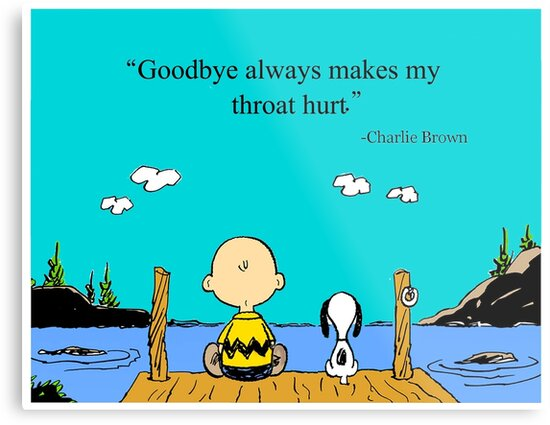
\includegraphics{PS01_source_files/mediabag/mp,550x550,gloss,fff.jpg}

}

\end{figure}

\begin{center}\rule{0.5\linewidth}{0.5pt}\end{center}

\begin{Shaded}
\begin{Highlighting}[]
\FunctionTok{sessionInfo}\NormalTok{()}
\end{Highlighting}
\end{Shaded}

\begin{verbatim}
R version 4.2.3 (2023-03-15)
Platform: x86_64-pc-linux-gnu (64-bit)
Running under: Red Hat Enterprise Linux 9.2 (Plow)

Matrix products: default
BLAS/LAPACK: /usr/lib64/libopenblasp-r0.3.21.so

locale:
 [1] LC_CTYPE=en_US.UTF-8       LC_NUMERIC=C              
 [3] LC_TIME=en_US.UTF-8        LC_COLLATE=en_US.UTF-8    
 [5] LC_MONETARY=en_US.UTF-8    LC_MESSAGES=en_US.UTF-8   
 [7] LC_PAPER=en_US.UTF-8       LC_NAME=C                 
 [9] LC_ADDRESS=C               LC_TELEPHONE=C            
[11] LC_MEASUREMENT=en_US.UTF-8 LC_IDENTIFICATION=C       

attached base packages:
[1] stats     graphics  grDevices utils     datasets  methods   base     

other attached packages:
[1] knitr_1.43

loaded via a namespace (and not attached):
 [1] compiler_4.2.2    fastmap_1.1.1     cli_3.6.1         tools_4.2.2      
 [5] htmltools_0.5.5   rstudioapi_0.15.0 yaml_2.3.7        rmarkdown_2.23   
 [9] jpeg_0.1-10       jsonlite_1.8.7    xfun_0.39         digest_0.6.33    
[13] rlang_1.1.1       png_0.1-8         evaluate_0.21    
\end{verbatim}

\begin{center}\rule{0.5\linewidth}{0.5pt}\end{center}



\end{document}
